\documentclass{standalone}
\usepackage{tikz}
\usetikzlibrary{patterns}
\usetikzlibrary{positioning}
\usetikzlibrary{patterns, positioning}
\usetikzlibrary{shapes.misc}
\usepackage[outline]{contour}
\contourlength{1.5pt} 
\usepackage[sfdefault]{ClearSans}

\begin{document}
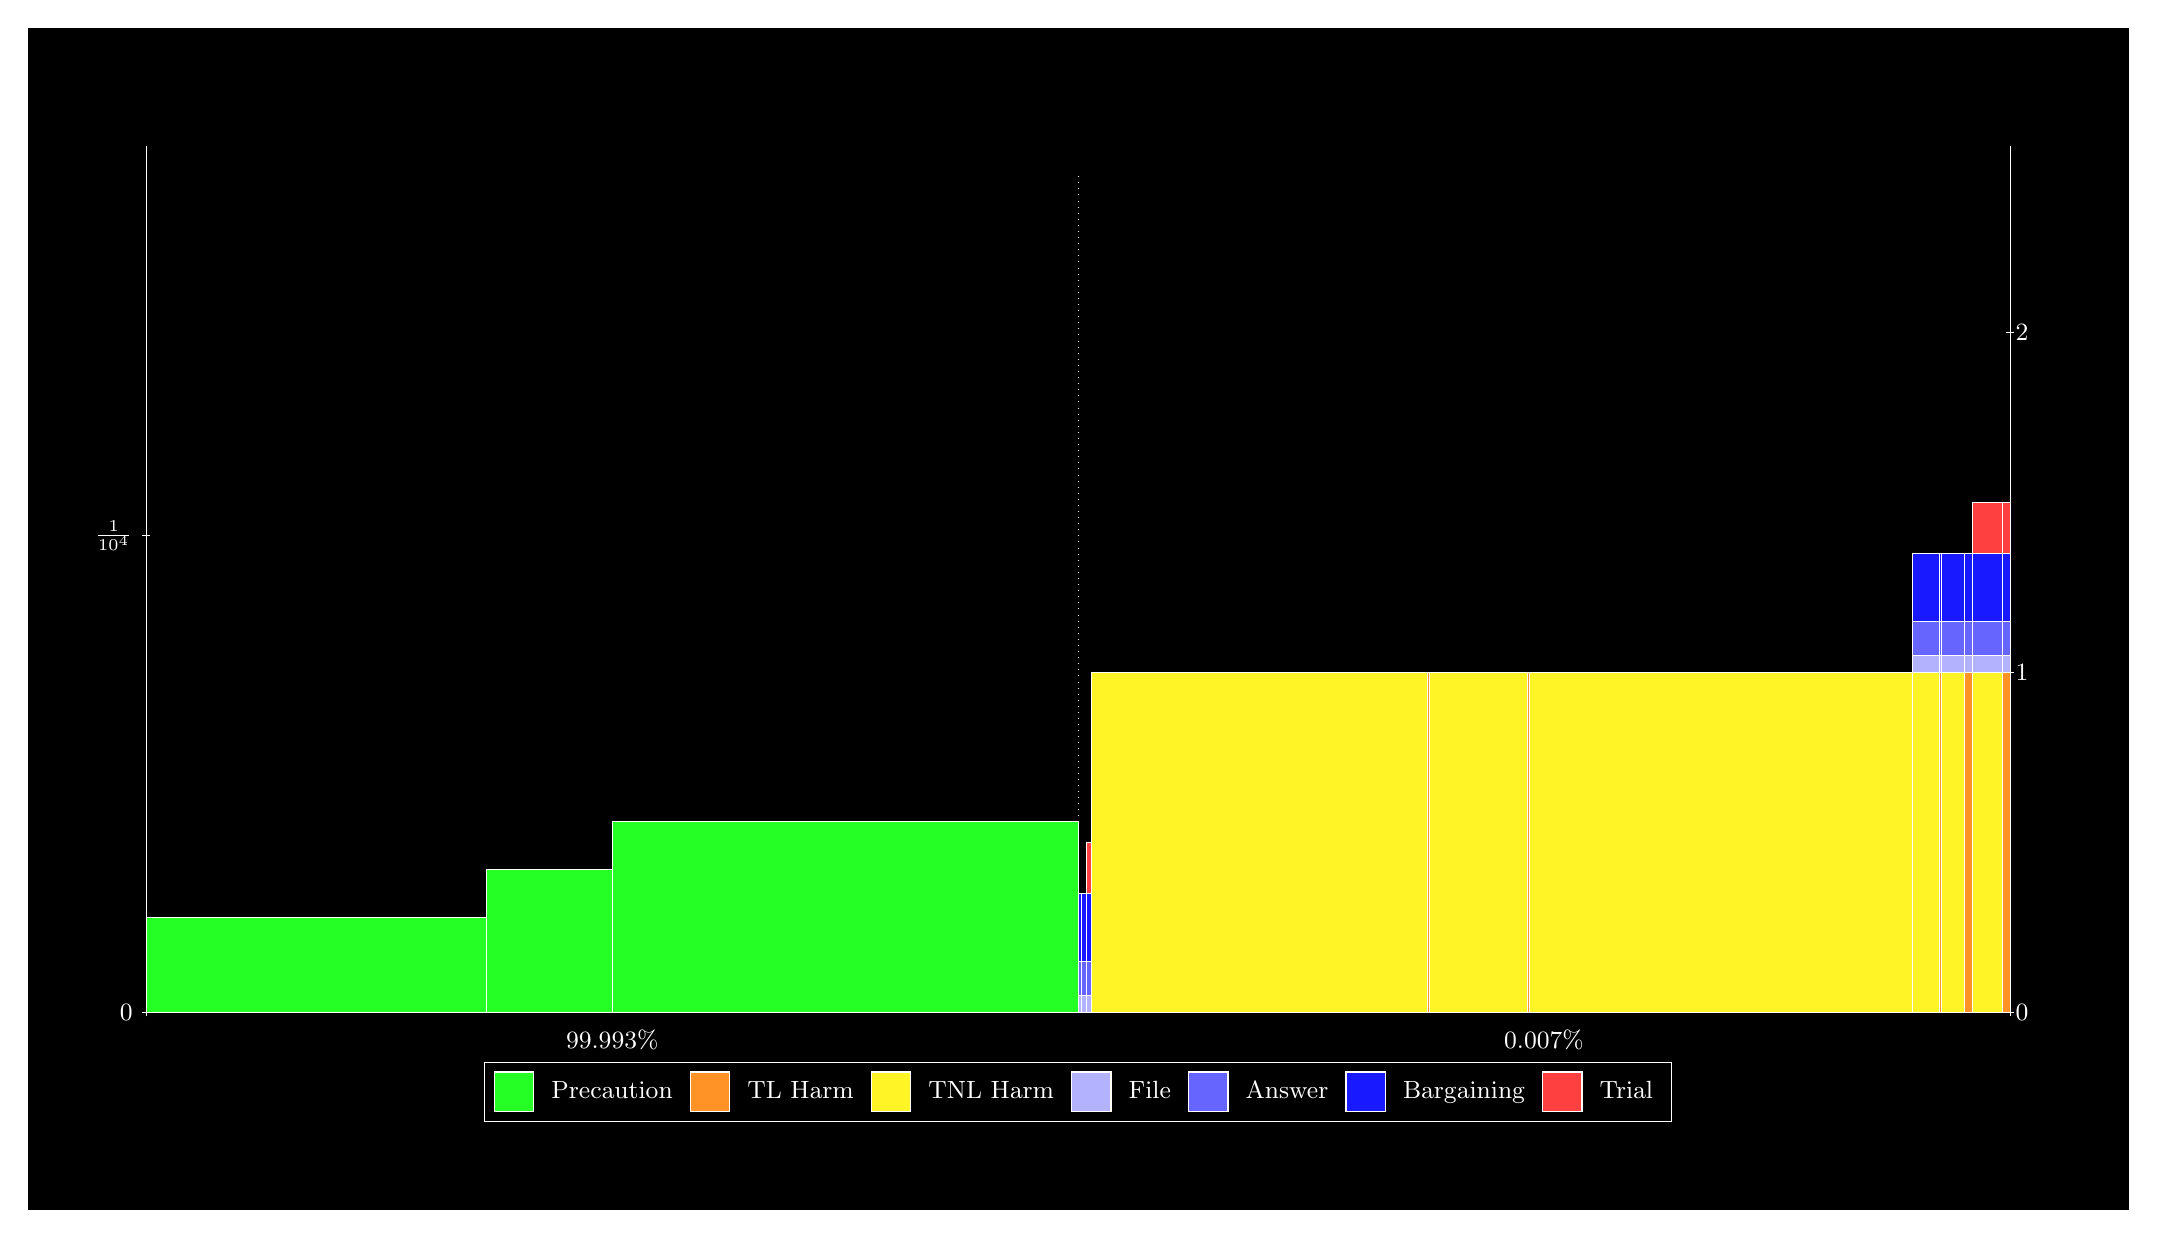
\begin{tikzpicture}
\draw[fill=black] (0,0) rectangle (26.667,15);
\draw[fill=green!85,draw=white,very thin] (1.5,2.5) rectangle (5.8206,3.7111);
\draw[fill=green!85,draw=white,very thin] (5.8206,2.5) rectangle (7.4166,4.3166);
\draw[fill=green!85,draw=white,very thin] (7.4166,2.5) rectangle (13.333,4.9222);
\draw[fill=green!85,draw=white,very thin] (13.333,2.5) rectangle (13.379,2.5001);
\draw[fill=blue!30,draw=white,very thin] (13.333,2.5001) rectangle (13.379,2.716);
\draw[fill=blue!60,draw=white,very thin] (13.333,2.716) rectangle (13.379,3.1477);
\draw[fill=blue!90,draw=white,very thin] (13.333,3.1477) rectangle (13.379,4.0112);
\draw[fill=green!85,draw=white,very thin] (13.379,2.5) rectangle (13.435,2.5001);
\draw[fill=blue!30,draw=white,very thin] (13.379,2.5001) rectangle (13.435,2.716);
\draw[fill=blue!60,draw=white,very thin] (13.379,2.716) rectangle (13.435,3.1477);
\draw[fill=blue!90,draw=white,very thin] (13.379,3.1477) rectangle (13.435,4.0112);
\draw[fill=green!85,draw=white,very thin] (13.435,2.5) rectangle (13.495,2.5001);
\draw[fill=blue!30,draw=white,very thin] (13.435,2.5001) rectangle (13.495,2.716);
\draw[fill=blue!60,draw=white,very thin] (13.435,2.716) rectangle (13.495,3.1477);
\draw[fill=blue!90,draw=white,very thin] (13.435,3.1477) rectangle (13.495,4.0112);
\draw[fill=red!75,draw=white,very thin] (13.435,4.0112) rectangle (13.495,4.6588);
\draw[fill=green!85,draw=white,very thin] (13.495,2.5) rectangle (17.773,2.5001);
\draw[fill=yellow!85,draw=white,very thin] (13.495,2.5001) rectangle (17.773,6.8174);
\draw[fill=green!85,draw=white,very thin] (17.773,2.5) rectangle (17.79,2.5001);
\draw[fill=orange!85,draw=white,very thin] (17.773,2.5001) rectangle (17.79,6.8174);
\draw[fill=green!85,draw=white,very thin] (17.79,2.5) rectangle (19.04,2.5001);
\draw[fill=yellow!85,draw=white,very thin] (17.79,2.5001) rectangle (19.04,6.8175);
\draw[fill=green!85,draw=white,very thin] (19.04,2.5) rectangle (19.057,2.5001);
\draw[fill=orange!85,draw=white,very thin] (19.04,2.5001) rectangle (19.057,6.8175);
\draw[fill=green!85,draw=white,very thin] (19.057,2.5) rectangle (23.922,2.5002);
\draw[fill=yellow!85,draw=white,very thin] (19.057,2.5002) rectangle (23.922,6.8175);
\draw[fill=green!85,draw=white,very thin] (23.922,2.5) rectangle (24.274,2.5001);
\draw[fill=yellow!85,draw=white,very thin] (23.922,2.5001) rectangle (24.274,6.8174);
\draw[fill=blue!30,draw=white,very thin] (23.922,6.8174) rectangle (24.274,7.0333);
\draw[fill=blue!60,draw=white,very thin] (23.922,7.0333) rectangle (24.274,7.465);
\draw[fill=blue!90,draw=white,very thin] (23.922,7.465) rectangle (24.274,8.3285);
\draw[fill=green!85,draw=white,very thin] (24.274,2.5) rectangle (24.298,2.5001);
\draw[fill=orange!85,draw=white,very thin] (24.274,2.5001) rectangle (24.298,6.8174);
\draw[fill=blue!30,draw=white,very thin] (24.274,6.8174) rectangle (24.298,7.0333);
\draw[fill=blue!60,draw=white,very thin] (24.274,7.0333) rectangle (24.298,7.465);
\draw[fill=blue!90,draw=white,very thin] (24.274,7.465) rectangle (24.298,8.3285);
\draw[fill=green!85,draw=white,very thin] (24.298,2.5) rectangle (24.593,2.5001);
\draw[fill=yellow!85,draw=white,very thin] (24.298,2.5001) rectangle (24.593,6.8175);
\draw[fill=blue!30,draw=white,very thin] (24.298,6.8175) rectangle (24.593,7.0333);
\draw[fill=blue!60,draw=white,very thin] (24.298,7.0333) rectangle (24.593,7.4651);
\draw[fill=blue!90,draw=white,very thin] (24.298,7.4651) rectangle (24.593,8.3285);
\draw[fill=green!85,draw=white,very thin] (24.593,2.5) rectangle (24.684,2.5001);
\draw[fill=orange!85,draw=white,very thin] (24.593,2.5001) rectangle (24.684,6.8175);
\draw[fill=blue!30,draw=white,very thin] (24.593,6.8175) rectangle (24.684,7.0333);
\draw[fill=blue!60,draw=white,very thin] (24.593,7.0333) rectangle (24.684,7.4651);
\draw[fill=blue!90,draw=white,very thin] (24.593,7.4651) rectangle (24.684,8.3285);
\draw[fill=green!85,draw=white,very thin] (24.684,2.5) rectangle (25.075,2.5001);
\draw[fill=yellow!85,draw=white,very thin] (24.684,2.5001) rectangle (25.075,6.8174);
\draw[fill=blue!30,draw=white,very thin] (24.684,6.8174) rectangle (25.075,7.0333);
\draw[fill=blue!60,draw=white,very thin] (24.684,7.0333) rectangle (25.075,7.465);
\draw[fill=blue!90,draw=white,very thin] (24.684,7.465) rectangle (25.075,8.3285);
\draw[fill=red!75,draw=white,very thin] (24.684,8.3285) rectangle (25.075,8.9761);
\draw[fill=green!85,draw=white,very thin] (25.075,2.5) rectangle (25.167,2.5001);
\draw[fill=orange!85,draw=white,very thin] (25.075,2.5001) rectangle (25.167,6.8174);
\draw[fill=blue!30,draw=white,very thin] (25.075,6.8174) rectangle (25.167,7.0333);
\draw[fill=blue!60,draw=white,very thin] (25.075,7.0333) rectangle (25.167,7.465);
\draw[fill=blue!90,draw=white,very thin] (25.075,7.465) rectangle (25.167,8.3285);
\draw[fill=red!75,draw=white,very thin] (25.075,8.3285) rectangle (25.167,8.9761);
\draw[white,very thin] (1.5,2.5) -- (1.5,13.5);
\draw[white,very thin] (1.45,2.5) -- (1.55,2.5);
\node[font=\small,text=white, anchor=east] at (1.45, 2.5) {0};
\draw[white,very thin] (1.45,8.5554) -- (1.55,8.5554);
\node[font=\small,text=white, anchor=east] at (1.45, 8.5554) {$\frac{1}{10^{4}}$};

\draw[white,dotted,very thin] (13.333,2.83) -- (13.333,13.17);
\draw[white,very thin] (25.167,2.5) -- (25.167,13.5);
\draw[white,very thin] (25.117,2.5) -- (25.217,2.5);
\node[font=\small,text=white, anchor=west] at (25.117, 2.5) {0};
\draw[white,very thin] (25.117,6.8173) -- (25.217,6.8173);
\node[font=\small,text=white, anchor=west] at (25.117, 6.8173) {1};
\draw[white,very thin] (25.117,11.135) -- (25.217,11.135);
\node[font=\small,text=white, anchor=west] at (25.117, 11.135) {2};

\draw[white,very thin] (1.5,2.5) -- (25.167,2.5);
\draw[white,very thin] (1.5,2.45) -- (1.5,2.55);
\node[font=\small,text=white, anchor=north] at (1.5, 2.45) {};
\draw[white,very thin] (25.167,2.45) -- (25.167,2.55);
\node[font=\small,text=white, anchor=north] at (25.167, 2.45) {};

\node[font=\small,text=white,anchor=south] at (7.4167, 1.9) {99.993\%};
\node[font=\small,text=white,anchor=south] at (19.25, 1.9) {0.007\%};
\draw (13.3333,2.5) node (B) {};
\begin{scope}[align=center]
\matrix[scale=0.5,draw=white,below=0.5cm of B,nodes={draw},column sep=0.1cm]{
\node[rectangle,draw,minimum width=0.5cm,minimum height=0.5cm,fill=green!85]{}; & \node[draw=none,font=\small,text=white]{Precaution}; &
\node[rectangle,draw,minimum width=0.5cm,minimum height=0.5cm,fill=orange!85]{}; & \node[draw=none,font=\small,text=white]{TL Harm}; &
\node[rectangle,draw,minimum width=0.5cm,minimum height=0.5cm,fill=yellow!85]{}; & \node[draw=none,font=\small,text=white]{TNL Harm}; &
\node[rectangle,draw,minimum width=0.5cm,minimum height=0.5cm,fill=blue!30]{}; & \node[draw=none,font=\small,text=white]{File}; &
\node[rectangle,draw,minimum width=0.5cm,minimum height=0.5cm,fill=blue!60]{}; & \node[draw=none,font=\small,text=white]{Answer}; &
\node[rectangle,draw,minimum width=0.5cm,minimum height=0.5cm,fill=blue!90]{}; & \node[draw=none,font=\small,text=white]{Bargaining}; &
\node[rectangle,draw,minimum width=0.5cm,minimum height=0.5cm,fill=red!75]{}; & \node[draw=none,font=\small,text=white]{Trial}; \\\\
};\end{scope}

\end{tikzpicture}
\end{document}